% ------------------------------------------------------------------------------
\documentclass[final, 12pt]{beamer}


% ========================================================================================
% Theme: inner, outer, font and colors
% ----------------------------------------------------------------------------------------
\usepackage[institute=FAU,
		  SecondLogo = template-art/TU-Berlin-Logo.svg,
            ThirdLogo = atelier/UMN2.png,
            SecondLogoFactor=0.3,
            ThirdLogoFactor=0.55,
            WordMarkRight=None,
		  size=a0,
            url = {tim.roith@fau.de},
            fontsize=18,
            fontbaselineskip=24,
		  ]{styles/beamerposterthemefau}
% ----------------------------------------------------------------------------------------
% Input and output encoding
\usepackage[T1]{fontenc}
\usepackage[utf8]{inputenc}
% ----------------------------------------------------------------------------------------
% Language settings
\usepackage[english]{babel}
% Package modifications
\setbeamertemplate{background}{}%
\setbeamerfont{title}{size=\LARGE,series=\bfseries}


% ========================================================================================
% Fonts
% - Helvet is loaded by styles/beamerfonts
% - We use serif for math environements
% - isomath is used for upGreek letters
% ----------------------------------------------------------------------------------------
\usepackage{isomath}
\usefonttheme[onlymath]{serif}
\usepackage{exscale}
\usepackage{anyfontsize}
\setbeamercolor{alerted text}{fg=BaseColor}
\setbeamerfont{alerted text}{series=\bfseries\boldmath}
% ----------------------------------------------------------------------------------------
% custom commands for symbols
\usepackage{styles/symbols}
\usepackage{subcaption}
\usepackage[capitalize, noabbrev]{cleveref}
\usepackage{pifont}
% todonotes packages
\usepackage{todonotes}
% ========================================================================================
% Setup for Titlepage
% ----------------------------------------------------------------------------------------
\title[]{Convergence rates for Lipschitz learning on very sparse graphs}
%\subtitle{ToDo}
\author[]{Leon Bungert\inst{1} \and Jeff Calder\inst{2} \and Tim Roith\inst{3}}
\institute[FAU]{%
\inst{1}Technical University of Berlin, Institute of Mathematics\and %
\inst{2}University of Minnesota, School of Mathematics\and %
\inst{3}Friedrich-Alexander-Universität Erlangen-Nürnberg, Department Mathematik}
\date{\today}


% ========================================================================================
% Bibliography
% ----------------------------------------------------------------------------------------

\usepackage{csquotes}
\usepackage[style=alphabetic, %alternatively: numeric, numeric-comp, and other from biblatex
			defernumbers=true,
			useprefix=true,%
			giveninits=true,%
			hyperref=true,%
			autocite=inline,%
			maxcitenames=5,%
			maxbibnames=20,%
			uniquename=init,%
			sortcites=true,% sort citations when multiple entries are passed to one cite command
			doi=false,%
			isbn=false,%
			url=false,%
			eprint=true,%
			backend=biber%
		   ]{biblatex}
\addbibresource{bibliography.bib}
\setbeamertemplate{bibliography item}[text]


% ========================================================================================
% Hyperref and setup
% ----------------------------------------------------------------------------------------
\usepackage{hyperref}
\hypersetup{
	colorlinks = true,
	final=true, 
	plainpages=false,
	pdfstartview=FitV,
	pdftoolbar=true,
	pdfmenubar=true,
	pdfencoding=auto,
	psdextra,
	bookmarksopen=true,
	bookmarksnumbered=true,
	breaklinks=true,
	linktocpage=true,
	urlcolor=BaseColor,
	citecolor=BaseColor,
	linkcolor=BaseColor
}


% ========================================================================================
% Additional packages
% ----------------------------------------------------------------------------------------



% ========================================================================================
% Various custom commands
% ----------------------------------------------------------------------------------------
\pdfsuppresswarningpagegroup=1 %solves the PDF inclusion problem
% Change color for cite locally
\newcommand{\colorcite}[3]{{\hypersetup{citecolor=#1}{\cite[#2]{#3}}}}
%\definecolor{fourierblue}{rgb}{0.78, 0.84, 0.93}

\usepackage{tikz}
\usetikzlibrary{shapes.arrows, fadings}
\newcommand{\trigo}[2]{#1\xrightarrow{\Delta}#2}
% colors
\definecolor{sky}{rgb}{0.31, 0.69, 0.99}
\definecolor{apple}{rgb}{0.33, 0.8, 0.14}
\definecolor{grape}{rgb}{0.99, 0.35, 0.34}
\definecolor{hpurp}{rgb}{0.87, 0., 1.}
\definecolor{orong}{rgb}{1.0, 0.55, 0.0}
\definecolor{ponk}{rgb}{1.0, 0.08, 0.58}
\definecolor{flamingopink}{rgb}{0.99, 0.46, 0.47}
\definecolor{teal}{rgb}{0.0, 0.5, 0.5}
\definecolor{brinkpink}{rgb}{0.98, 0.38, 0.5}
\definecolor{carnationpink}{rgb}{1.0, 0.65, 0.79}

\newcommand{\nc}{\color{black}}
\colorlet{fourierblue}{sky}
\usetikzlibrary{arrows}
\usetikzlibrary{calc,arrows.meta,fadings}
\renewcommand\fbox{\fcolorbox{sky}{white}}
% ----------------------------------------------------------------------------------------
% ========================================================================================
% The main document
% ----------------------------------------------------------------------------------------
\begin{document}
\begin{frame}[t]{-}
%
% >>>>>>>>>>>>>>>>>>>>>>>>>>>>>>>>>>>>>>>>>>>>>>>>>>>>>>>>>>>
% Dimensions
% <<<<<<<<<<<<<<<<<<<<<<<<<<<<<<<<<<<<<<<<<<<<<<<<<<<<<<<<<<<
\newdimen\topWidth
\newdimen\topHeight
\newdimen\seplineHeight
\topWidth=.31\textwidth
\topHeight=.22\textheight
\seplineHeight=60pt
\setbeamercolor{block body}{bg=sky!10!white,fg=black}
\setbeamercolor{block poster title}{bg=sky!70!white,fg=white}
%
%
%\vfill%
\begin{minipage}[t][\topHeight][t]{\topWidth}%
{\color{BaseDarkColor}\usebeamerfont{block title} Semi-supervised Learning}\\%
Given a finite set of $n$ points $\domain_n\nc\subset\domain\subset\R^d$ with labels $\color{grape}\vec g\nc:\constr_n\nc\subset\domain_n\rightarrow\R$, find a function
\begin{block}{}%
\belowdisplayskip=0pt%
\abovedisplayskip=0pt%
\begin{align*}%
\vec u:\domain_n\nc\to\R,\;\text{ s.t. }\vec u=\color{grape}\vec g \nc\text{ on } \constr_n\nc.
\end{align*}%
\end{block}%
%
\begin{center}%
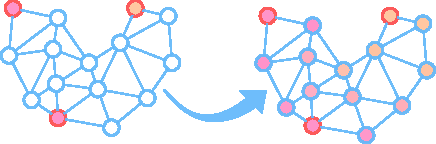
\includegraphics[width=.8\textwidth]{atelier/SSL.pdf}%
\end{center}%
%
{\noindent\color{BaseDarkColor}\usebeamerfont{block title}%
Weighted Graphs}\\%
We model the data as a \alert{weighted graph} $(\domain_n,w_n)$ with edge weights given by
\begin{align*}
w_n(x,y):=
\eta(\abs{x-y}/\scaling_n),\quad x,y\in\domain_n\nc.
\end{align*}
Here $\scaling_n\nc>0$ is a \color{apple}\textbf{scaling parameter}\nc{} and \linebreak $\eta:[0,\infty)\rightarrow[0,\infty)$ is a kernel function.
%
\end{minipage}%
%}%
%
%
\hfill%
%
%
\begin{minipage}[t][\topHeight][t]{0.33\textwidth}%
{\color{BaseDarkColor}\usebeamerfont{block title} Laplacian Learning}\\%
Laplacian learning for $p<\infty$ involves the energy
\begin{align*}
\vec E_p^{w_n}(\vec u) = \sum_{x,y\in\domain_n}w_n(x,y)^p|\vec u(y)-\vec u(x)|^p
\end{align*}
%
and the graph Laplacian
%
{\small%
\begin{align*}
\Delta^{w_n}_p \vec u(x):= \sum_{y\in\domain_n} w_n(x,y)^p \abs{\vec u(y) - \vec u(x)}^{p-2} \left( \vec u(y) - \vec u(x) \right)
\end{align*}
}%
%
%
which yields the equivalent problems:
\vspace{15pt}

%
\begin{minipage}{.45\textwidth}%
\begin{block}{}%
\vbox to 4cm {%
\belowdisplayskip=0pt%
\abovedisplayskip=0pt%
\begin{gather*}
\min_{\vec u} \vec{E}^{w_n}_p (\vec u),\\
\text{ s.t. } \vec u = \color{grape}\vec g\nc \text{ on } \constr_n.
\end{gather*}\vfill}%
\end{block}
\end{minipage}%
\hfill%
$\Leftrightarrow$
\hfill%
\begin{minipage}{.45\textwidth}%
\begin{block}{}
\vbox to 4cm {%
\belowdisplayskip=0pt%
\abovedisplayskip=0pt%
\begin{align*}
\Delta^{w_n}_p\vec u&= 0\text{ in } \domain_n\setminus\constr_n,\\
\vec u &= \color{grape}\vec g\nc \text{ on } \constr_n.
\end{align*}\vfill}%
\end{block}
%
\end{minipage}%
\vspace{.1em}

%
\begin{minipage}{.5\textwidth}%
\centering%
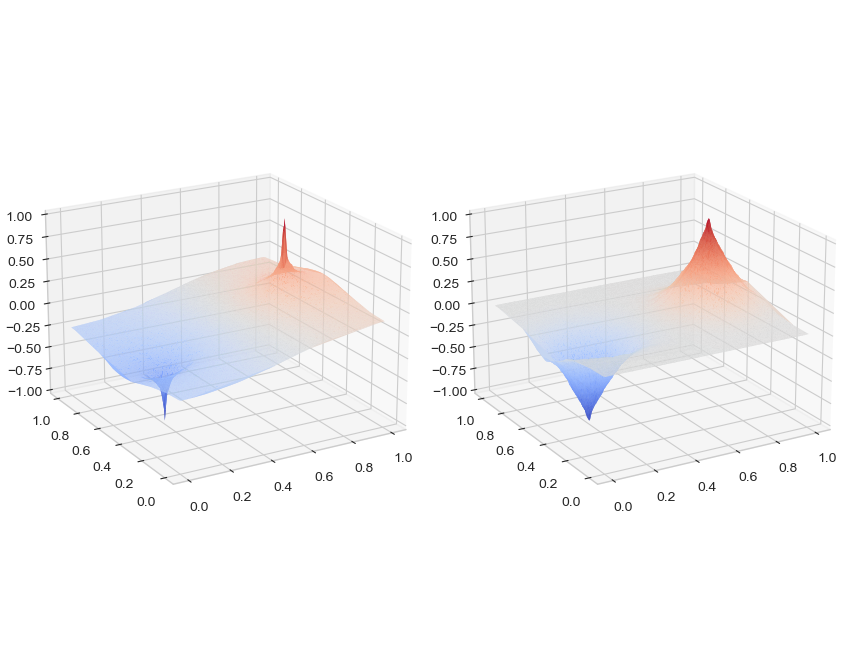
\includegraphics[width=.7\textwidth, trim={0cm 3cm 11cm 4cm}, clip]{atelier/2Dex_50000.png}%
\end{minipage}%
\begin{minipage}{.5\textwidth}%
\alert{Drawback:} In the infinite data limit this problem is only well-posed if $p>d$.
\end{minipage}%
%
%
\vfill%
%
\end{minipage}%
%
%
\hfill%
%
%
\begin{minipage}[t][\topHeight][t]{\topWidth}%
{\color{BaseDarkColor}\usebeamerfont{block title} Lipschitz Learning}\\%
In the limit $p\to\infty$ we obtain the energy
\begin{align*}
\vec E_\infty^{w_n}(\vec u) = \max_{x,y\in\domain_n}w_n(x,y)|\vec u(y)-\vec u(x)|
\end{align*}
%
and the graph infinity Laplacian
%
{\small%
\begin{align*}
\Delta^{w_n}_\infty \vec u(x)
&:= 
\max_{y\in\domain_n} w_n(x,y) \left(\vec u(y) - \vec u(x)\right)
\\
&\qquad
+ 
\min_{y\in\domain_n} w_n(x,y) \left(\vec u(y) - \vec u(x)\right).
\end{align*}}%
%
The associated problems are not equivalent.
%
\begin{minipage}{.45\textwidth}%
\begin{block}{}%
\vbox to 4cm {%
\belowdisplayskip=0pt%
\abovedisplayskip=0pt%
\begin{gather*}
\min_{\vec u} \vec{E}^{w_n}_\infty (\vec u),\\
\text{ s.t. } \vec u = \color{grape}\vec g\nc \text{ on } \constr_n.
\end{gather*}\vfill}%
\end{block}
\end{minipage}%
\hfill%
$\Leftarrow$%
\hfill%
%
\begin{minipage}{.45\textwidth}%
\begin{block}{}
\vbox to 4cm {%
\belowdisplayskip=0pt%
\abovedisplayskip=0pt%
\begin{align*}
\Delta^{w_n}_\infty\vec u&= 0\text{ in } \domain_n\setminus\constr_n,\\
\vec u &= \color{grape}\vec g \nc \text{ on } \constr_n.
\end{align*}\vfill}%
\end{block}
\end{minipage}%
%
\vspace{1em}%

\begin{minipage}{.5\textwidth}%
\centering%
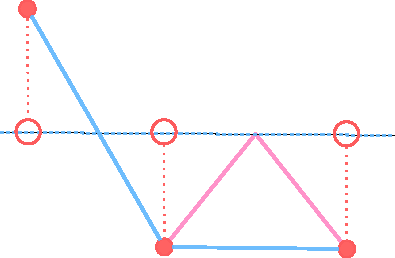
\includegraphics[width=.7\textwidth]{atelier/amle.pdf}%
\end{minipage}%
\begin{minipage}{.5\textwidth}%
Minimizing $\vec E_\infty^{w_n}$ does not admit unique solutions: the blue line shows the~\alert{AMLE}.
\end{minipage}%

\end{minipage}%
\hfill%%
\newdimen\midWidth
\newdimen\midHeight
\midWidth=.31\textwidth
\midHeight=.17\textheight
% The following empty line is intentional!

% >>>>>>>>>>>>>>>>>>>>>>>>>>>>>>>>>>>>>>>
% Seperation Line
% <<<<<<<<<<<<<<<<<<<<<<<<<<<<<<<<<<<<<<<
%\vfill%
\begin{minipage}[t][\seplineHeight][b]{\textwidth}%
%\fbox{%
\vbox to \seplineHeight{%
\vfill%
\begin{center}%
\textcolor{sky}{%
\rule{\textwidth}{.2mm}}%
\end{center}%
\vfill%
}%
%}%
\end{minipage}%
\noindent%

\begin{minipage}[b][\midHeight][t]{\topWidth}%
{\color{BaseDarkColor}\usebeamerfont{block title} Graph Resolution}\\%
Using the Hausdorff distance
% 
\begin{align*}
d_H(A,B)=\sup_{x\in A} \dist(x,B) \vee \sup_{x\in B} \dist(x,A)
\end{align*}
we consider the \color{ponk}\textbf{graph resolution}\nc:
\begin{align*}
\gres_n=
d_H(\domain_n, \domain) 
\vee d_H(\constr_n, \constr).
\end{align*}
%
\nc
%
%
%
{\color{BaseDarkColor}\usebeamerfont{block title} \noindent Local Convexity}%

%
%
%
\begin{minipage}{.4\textwidth}%
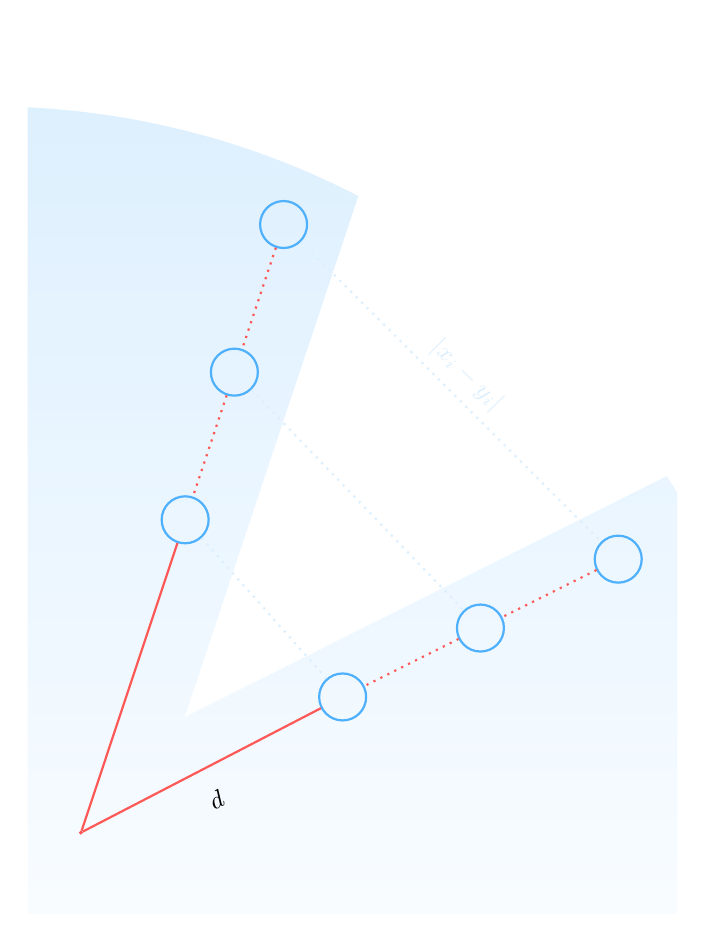
\begin{tikzpicture}[scale=2.5]
\begin{scope}
\clip(1.2,1.0) rectangle (4.5,5.5);
\clip(1.0,1.0) circle (4.1cm);

\begin{scope}
%\path [scope fading=my fading,fit fading=false] (1,0) rectangle (8,8);
\path[fill=sky!30, draw = none, path fading=south] plot coordinates {(0,0)(0,8)(4,8)(2,2)(6,4)(8,0)} node at (1.8,1.7) {};
\end{scope}
\begin{scope}[every node/.style={circle,thick,sky,draw, inner sep=6pt}]
\node (X1) at (2.5,4.5) {};
\node (X2) at (2.25,3.75) {};
\node (X3) at (2.0,3.0) {};
\node (Y1) at (4.2,2.8) {};
\node (Y2) at (3.5,2.45) {};
\node (Y3) at (2.8,2.1) {};
\end{scope}
\node[circle,fill,draw,grape,inner sep=0pt] (Z) at ($(X1) - 1.03*(1,3)$) {};
%\node[circle,fill=faulnat,inner sep=0,text=sky] (J) at (1.5,5.2) {$x$};

\begin{scope}[every path/.style={grape,dotted,thick}]
\path (X1) edge (X2);
\path (X2) edge (X3);
\path (Y1) edge (Y2);
\path (Y2) edge (Y3);
\end{scope}
%\path[draw=sky] [-] (B) edge (J2);
\path[grape,thick] (X3) edge (Z);
\path[grape,thick] (Y3) edge node[sloped,below=5pt,pos=0.5] {\small\nc$d_{\domain}$} (Z);
\begin{scope}[every path/.style={sky!20,dotted, thick}]
\path (X1) edge  node[sloped, above] {\small$|x_i-y_i|$} (Y1);
\path (X2) edge (Y2);
\path (X3) edge (Y3);
\end{scope}
\end{scope}
\end{tikzpicture}
\end{minipage}%
%
%
\begin{minipage}{.6\textwidth}%
We assume that $\domain$ is \alert{locally convex}, i.e., $\forall x,y\in\domain$:
\begin{align*}
d_\domain(x,y) \leq \abs{x-y} + \phi(\abs{x-y})
\end{align*}
where ${\phi(\gscale)}\ll{\gscale}$ as $\gscale\to 0$.

$\Rightarrow$ No sharp internal corners.
\end{minipage}%
\end{minipage}%
%
%
%
\hfill%
%
%
%
%\fbox{%
\begin{minipage}[b][\midHeight][t]{\topWidth}%
\tikzfading[name=fade out, 
    inner color=transparent!0,
    outer color=transparent!60]
\hspace*{2em}\raisebox{-17em}{%
\begin{tikzpicture}[scale=2.7]
\draw[fill=sky!10, draw = none, thick, dashed] plot [smooth cycle] coordinates {(-1,.1)(-0.2,5.5)(4,4.9)(4.5,3)(6,1)(4,-0.5)(2,-1)} node at (1.8,1.7) {};
%
\node (F) at (3.5,1.5) {};
\fill[apple!20,path fading = fade out] (F) circle (57pt);
%
\begin{scope}[every node/.style={circle,very thick,sky,draw,inner sep=6pt}]
\node (A) at (0.7,1.9) {};
\node (B) at (1.8,1.3) {};	
\node[grape] (C) at (2.,5.2) {};
\node[grape] (D) at (-0.7,2.5) {};
\node[] (F) at (F) {};
\node[grape] (G) at (-0.2,1.5) {} ;
\node[grape] (E) at (0.2,3.8) {};
\node (H) at (2.8,4) {};
\node (I) at (2.5,3.) {};
\end{scope}

\draw[->,>=Latex,apple, thick] (F) -- 
    +(-135:57pt) node[midway,below,sloped]{\small\nc$\sim \scaling_n$};

\node (Omega) at (0,5) {$\domain$};
\node (Omegan) at (3.5,4.2) {$\domain_n$};
\node (On) at ($(E)+(0.5,0.5)$) {$\mathbin{\constr_n}$};

% boundary
\begin{scope}
\clip (-0.5,-1.2) rectangle (3,6);
\draw[fill=none, draw = grape, very thick, dashed] plot [smooth cycle] coordinates {(-1,.1)(-0.2,5.5)(4,4.9)(4.5,3)(6,1)(4,-0.5)(2,-1)} node at (2.2,5.7) {$\mathbin{\constr}$};
\end{scope}
\draw[grape,very thick,dashed] plot [smooth] coordinates {(-0.5,-0.44)(-.7,.2)(0,3.5)(1.5,2.5)(2,3.0)};
%
\begin{scope}[every path/.style={sky}]
\path [-] (A) edge (B);
\path [-] (A) edge (E);
\path [-] (A) edge (D);
\path [-] (A) edge (G);
\path [-] (D) edge (G);
\path [-] (C) edge (H);
\path [-] (D) edge (E);
\path [-] (B) edge (F);
\path [-] (I) edge (F);
\path [-] (I) edge (B);
\path [-] (I) edge (H);
\end{scope}
%
\node[circle,very thick,ponk,draw, fill, inner sep=3pt] (J) at (0.5,-0.5) {};
\path[draw=ponk, dotted, very thick] [-] (B) edge node[midway,below, sloped] {\small$\gres_n$} (J) ;
\end{tikzpicture}}%
%
\end{minipage}%
%}%
%
%
%
%
%
%
\hfill%
%
\begin{minipage}[b][\midHeight][t]{\topWidth}%
{\color{BaseDarkColor}\usebeamerfont{block title} $\Gamma$-Convergence}\\%
%
Considering the functionals 
%
\begin{align*}
E_\infty^{w_n}(\vec u) &:= \frac{1}{\scaling_n}\ \vec E_\infty^{w_n}(\vec u)  &&+ \color{grape} \textbf{constraint},\\
\func_\infty(u) &:= \norm{\nabla u}_{L^\infty(\domain)}
&&+ \color{grape} \textbf{constraint},
\end{align*}
%
%
we prove in \cite{roith2022continuum}:
%
\begin{itemize}
\item $E_\infty^{w_n}\xrightarrow[]{\hspace*{.5cm}\Gamma\hspace*{.5cm}}
\sigma_\eta~\func_\infty$ in a suitable topology,
\item $\sup_{n\in\N}E_\infty^{w_n}(\vec u_n)<\infty$ and boundedness imply that $(\vec u_n)_{n\in\N}$ is relatively compact.
\end{itemize}
%
Here we assume the \alert{weakest scaling}%, i.e., $\color{apple}\scaling_n\nc$ is a null sequence with 
\begin{align*}
%\frac{\color{ponk}\gres_n}{\color{apple}\scaling_n\nc}\longrightarrow 0.
\gres_n\ll\scaling_n\ll 1.
\end{align*}
\end{minipage}%
% The following empty line is intentional!

% >>>>>>>>>>>>>>>>>>>>>>>>>>>>>>>>>>>>>>>>>>>>>>>>>>>>>>>>>>>
% Seperation Line
% <<<<<<<<<<<<<<<<<<<<<<<<<<<<<<<<<<<<<<<<<<<<<<<<<<<<<<<<<<<
%\vfill%
\begin{minipage}[t][\seplineHeight][b]{\textwidth}%
%\fbox{%
\vbox to \seplineHeight{%
\vfill%
\begin{center}%
\textcolor{sky}{%
\rule{\textwidth}{.2mm}}%
\end{center}%
\vfill%
}%
%}%
\end{minipage}%
\begin{minipage}[b][\midHeight][t]{.48\textwidth}%
{\color{BaseDarkColor}\usebeamerfont{block title} The $\infty$-Laplacian and AMLEs}\\%
%
For $\Delta_\infty u(x) := \langle \nabla u(x), \nabla^2 u(x) \nabla u(x)\rangle$ we consider the problems:\vspace{-1em}\\
%
%
\begin{minipage}[t]{.3\textwidth}%
\begin{block}{$\infty$-Laplacian}
\vbox to 6cm{%
\small%
\begin{align*}
\Delta_\infty u &= 0\quad\text{in }\domain,\\
u&=\color{grape} g\nc\quad\text{on }\constr,\\
\frac{\partial u}{\partial\nu} &= 0 \quad\text{on }\partial\domain\setminus\constr.
\end{align*}
\vfill}%
\end{block}
\end{minipage}%
%
\hfill%
%
\begin{minipage}[t]{.33\textwidth}%
%
\begin{block}{AMLE}
\vbox to 6cm{%
\small%
\begin{align*}
\Lip_{d_\domain}(u; \overline{V}) &= \Lip_{d_\domain}(u, \partial V),\\
u &= \color{grape} g\nc\quad\text{on }\constr,
\end{align*}
for all open and connected sets  $V\subset \overline{\domain}\setminus\constr.$
\vfill%
}%
\end{block}
\end{minipage}%
%
\hfill%
%
\begin{minipage}[t]{.33\textwidth}%
%
\begin{block}{CDF}
\vbox to 6cm{%
\small%
$h_\pm := \pm u - a \abs{\cdot - y}$ satisfies
\abovedisplayskip=0pt%
\begin{align*}
\max_{\overline V}h_\pm &= 
\max_{\partial V} h_\pm,
\end{align*}
% $\forall X\subset\subset\domain$, $y\in\domain\setminus X$, and $a\geq 0$.
for all such sets $V\subset \overline{\domain}\setminus\constr$, $y\in\overline{\domain}\setminus V$, and $a\geq 0$.
\vfill%
}%
\end{block}
\end{minipage}
%
\begin{itemize}
\setlength\itemsep{3pt}
\item Regular $\partial\domain$: $\infty$-harmonic $\Leftrightarrow$ AMLE $\Leftrightarrow$ CDF. 
\item AMLE and CDF can be generalized to the graph, using the distance
%
\small
\begin{align*}
d_n(x,y) 
:=
\inf
\left\lbrace
\sum_{i=1}^{m-1} \frac{1}{\omega_n(p_{i+1},p_i)}
\st 
m \in \N,\,
p \in \domain_n^m,\,
p_1=x,\,p_m = y
\right\rbrace.
\end{align*}
%
\end{itemize}
%
\begin{block}{}%
\cite{bungert2021uniform}: 
$\Delta_\infty^{w_n}\vec u=0$ $\;\Rightarrow\;$ $\vec u$ is graph AMLE and fulfills graph CDF.
\end{block}%
\end{minipage}%
%
%
\hfill%
%
%
\begin{minipage}[b][\midHeight][t]{.49\textwidth}%
{\color{BaseDarkColor}\usebeamerfont{block title} Meeting in the Middle}\\
Larger length scale $\nlscale>0$: consider \color{orong}\textbf{homogenized operator}\nc
%
\begin{align*}
\small%
\nlscale^2 \Delta_\infty^\nlscale u(x) &:= \sup_{y\in \closure B(x;\nlscale)}(u(y)-u(x)) + \inf_{y\in \closure B(x;\nlscale)}(u(y)-u(x)).
\end{align*}
%
\fbox{\begin{minipage}[b][9cm][t]{.4\textwidth}%
\small\textbf{Local to Non-Local}: CDF implies \cite{armstrong2010easy} for
\begin{align*}
%u^\nlscale(x) = \sup_{\overline B(x;\nlscale)}u\quad\text{and}\quad
u_\nlscale(x) = \inf_{\overline B(x;\nlscale)}u
\end{align*}
that
\begin{align*}
% -\Delta_\infty u &\leq 0 \Rightarrow -\Delta_\infty^\nlscale u^\nlscale\leq 0,
% \\
-\Delta_\infty u &\geq 0 \Rightarrow -\Delta_\infty^\nlscale u_\nlscale \geq 0.
\end{align*} 
\end{minipage}}%
%
\hfill%
%
\fbox{\begin{minipage}[b][9cm][t]{.52\textwidth}
\small\textbf{Discrete to Non-Local}:
CDF on the graph implies \cite{bungert2021uniform} for $u_n^\nlscale(x):=\max_{y\in \overline B(x;\nlscale)\cap\domain_n}\vec u_n(y)$ that
%
\begin{align*}
-\Delta_\infty^{w_n}\vec u_n \leq 0
\Rightarrow
-\Delta_\infty^\nlscale u_n^{\nlscale}
\lesssim 
\frac{{r_\nlscale}}{\nlscale}
+
\frac{\gscale_n}{\nlscale^2},
\end{align*}
%
where
%
\begin{align*}
r_\nlscale(x) := 
\frac{\sup_{y\in \overline B(x,\nlscale)\cap \domain_n}d_n(x,y)}{\inf_{y\in \domain_n\setminus \overline B(x,2\nlscale-\gscale_n)}d_n(x,y)}
-
\frac12.
\end{align*}
\end{minipage}}%
%

\vbox to 6cm{%
\begin{block}{}
\small%
\textbf{Non-Local}: Using \alert{strictness perturbations} and Lipschitzness, and swapping signs we obtain
\begin{align}\label{eq:estimate}\tag{rate}
\sup_{\Omega_n}\abs{\vec u_n - u} \lesssim \nlscale +  \sqrt[3]{\frac{r_\nlscale}{\nlscale} + \frac{\gscale_n}{\nlscale^2}}.
\end{align}
\end{block}
}%
%

\end{minipage}
% >>>>>>>>>>>>>>>>>>>>>>>>>>>>>>>>>>>>>>>>>>>>
% Dimensions
% <<<<<<<<<<<<<<<<<<<<<<<<<<<<<<<<<<<<<<<<<<<<
\newdimen\bottomHeight%
\bottomHeight=.15\textheight%
% The following empty line is intentional!

% >>>>>>>>>>>>>>>>>>>>>>>>>>>>>>>>>>>>>>>
% Seperation Line
% <<<<<<<<<<<<<<<<<<<<<<<<<<<<<<<<<<<<<<<
%\vfill%
\begin{minipage}[t][\seplineHeight][b]{\textwidth}%
%\fbox{%
\vbox to \seplineHeight{%
\vfill%
\begin{center}%
\textcolor{sky}{%
\rule{\textwidth}{.2mm}}%
\end{center}%
\vfill%
}%
%}%
\end{minipage}%
\noindent%

\begin{minipage}[b][\midHeight][t]{.34\textwidth}%
{\color{BaseDarkColor}\usebeamerfont{block title} Key Insight from \cref{eq:estimate}:}
%
\begin{block}{}
\centering%
\textit{%
\enquote{Ratio convergence rates for the distance function imply convergence rates for AMLEs.}}
\end{block}
%
In \cite{bungert2021uniform} we prove:
\abovedisplayskip=0pt%
\belowdisplayskip=0pt%
\begin{align*}
\abs{x-y} \leq 
\sigma_\eta d_n(x,y)
\leq 
\left(1 + C \frac{\gres_n}{\gscale_n}\right) 
\abs{x-y} + \tau_\eta \, \gscale_n,
\end{align*}
where
$\sigma_\eta := \sup_{t>0}\eta(t)t$ and $\tau_\eta := \sup_{t>0}\sigma_\eta\eta(t)^{-1}-t.$
%
\vspace{.2em}

\fbox{%
\begin{minipage}[b][4cm][c]{\textwidth}%
\textbf{Sparse regime}: If $\gres_n\lesssim\gscale_n\lesssim\gres_n^{\frac{5}{9}}$ the rate is $\left({\gres_n}/{\gscale_n}\right)^{\frac{1}{4}}$.\\
\textbf{Dense regime}: If $\gscale_n\gtrsim\gres_n^{\frac{5}{9}}$ the rate is $\gscale_n^{\frac{1}{5}}$.
\end{minipage}}%
\vspace{.5em}
{\color{BaseDarkColor}\usebeamerfont{block title} \noindent What about $\gscale_n\sim\gres_n$? Percolation!}\\
\small
On a unit intensity Poisson Point Process $X\subset\R^d$ and for $h>0$ let $\Pi_h(x,y)$ be the set of admissible paths and
%
\begin{align*}
T_s := d_{h_s}(0,s e_1) := \inf 
\left\lbrace\sum_{i=1}^{\operatorname{len}(p)-1} \abs{p_{i+1}-p_{i}} \st 
p\in\Pi_{h_s}(0,s e_1)
\right\rbrace.
\end{align*}
%
\alert{Important}: Replace $T_s$ by distance $T_s^\prime$ on an \alert{enriched process} $\mathcal{X}_s$.
\end{minipage}%
%
%
\hfill%
%
%
\begin{minipage}[b][\midHeight][t]{.31\textwidth}%
%
\begin{minipage}{\textwidth}
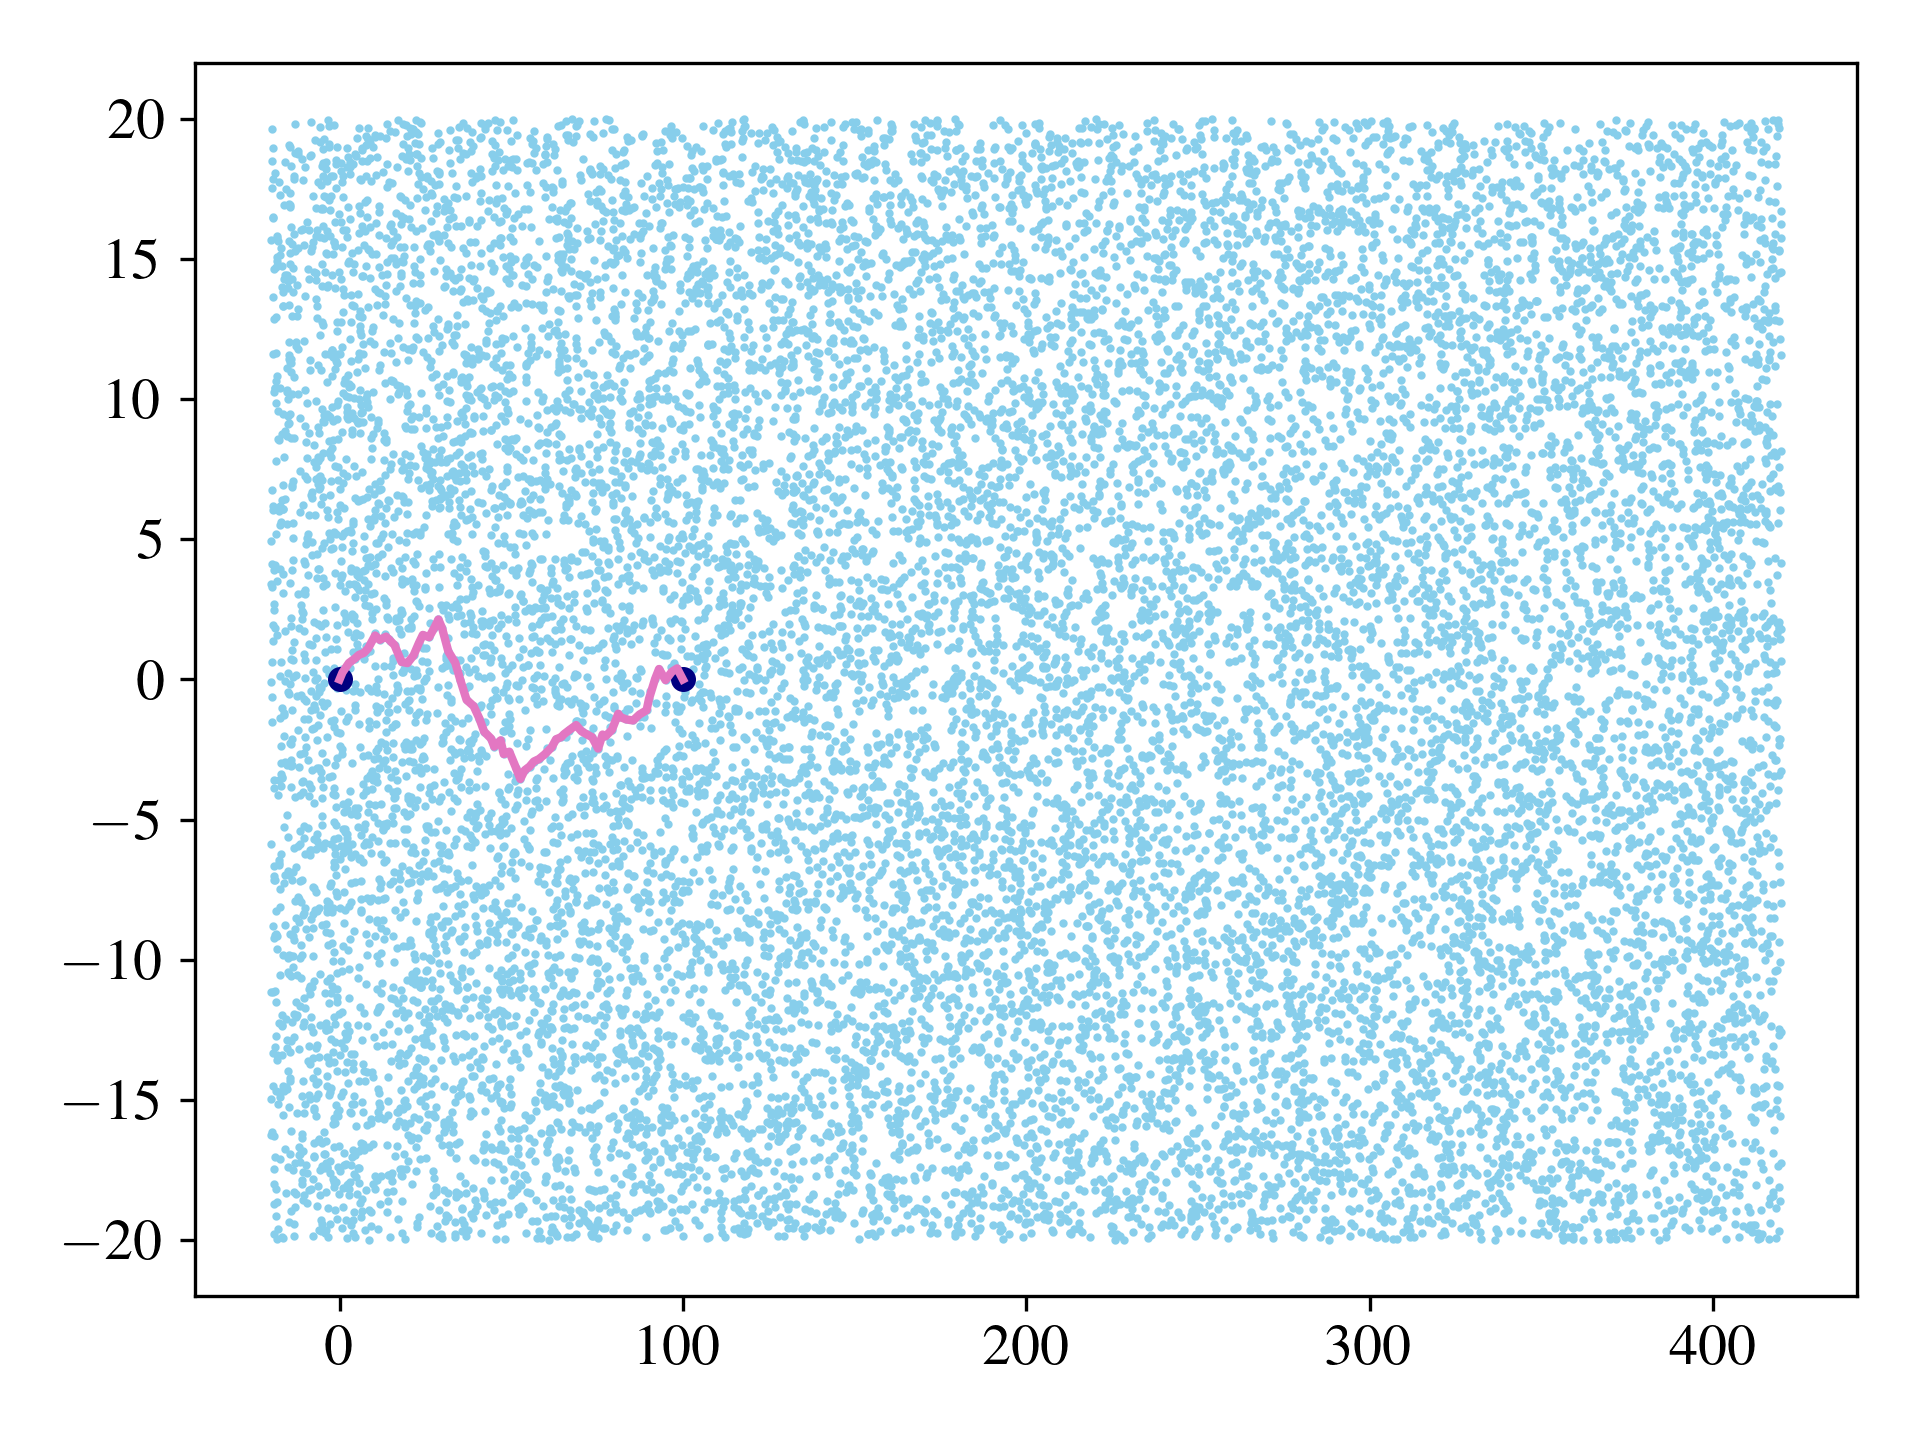
\includegraphics[width=0.3\textwidth]{atelier/path_2d_s-100}
\hfill
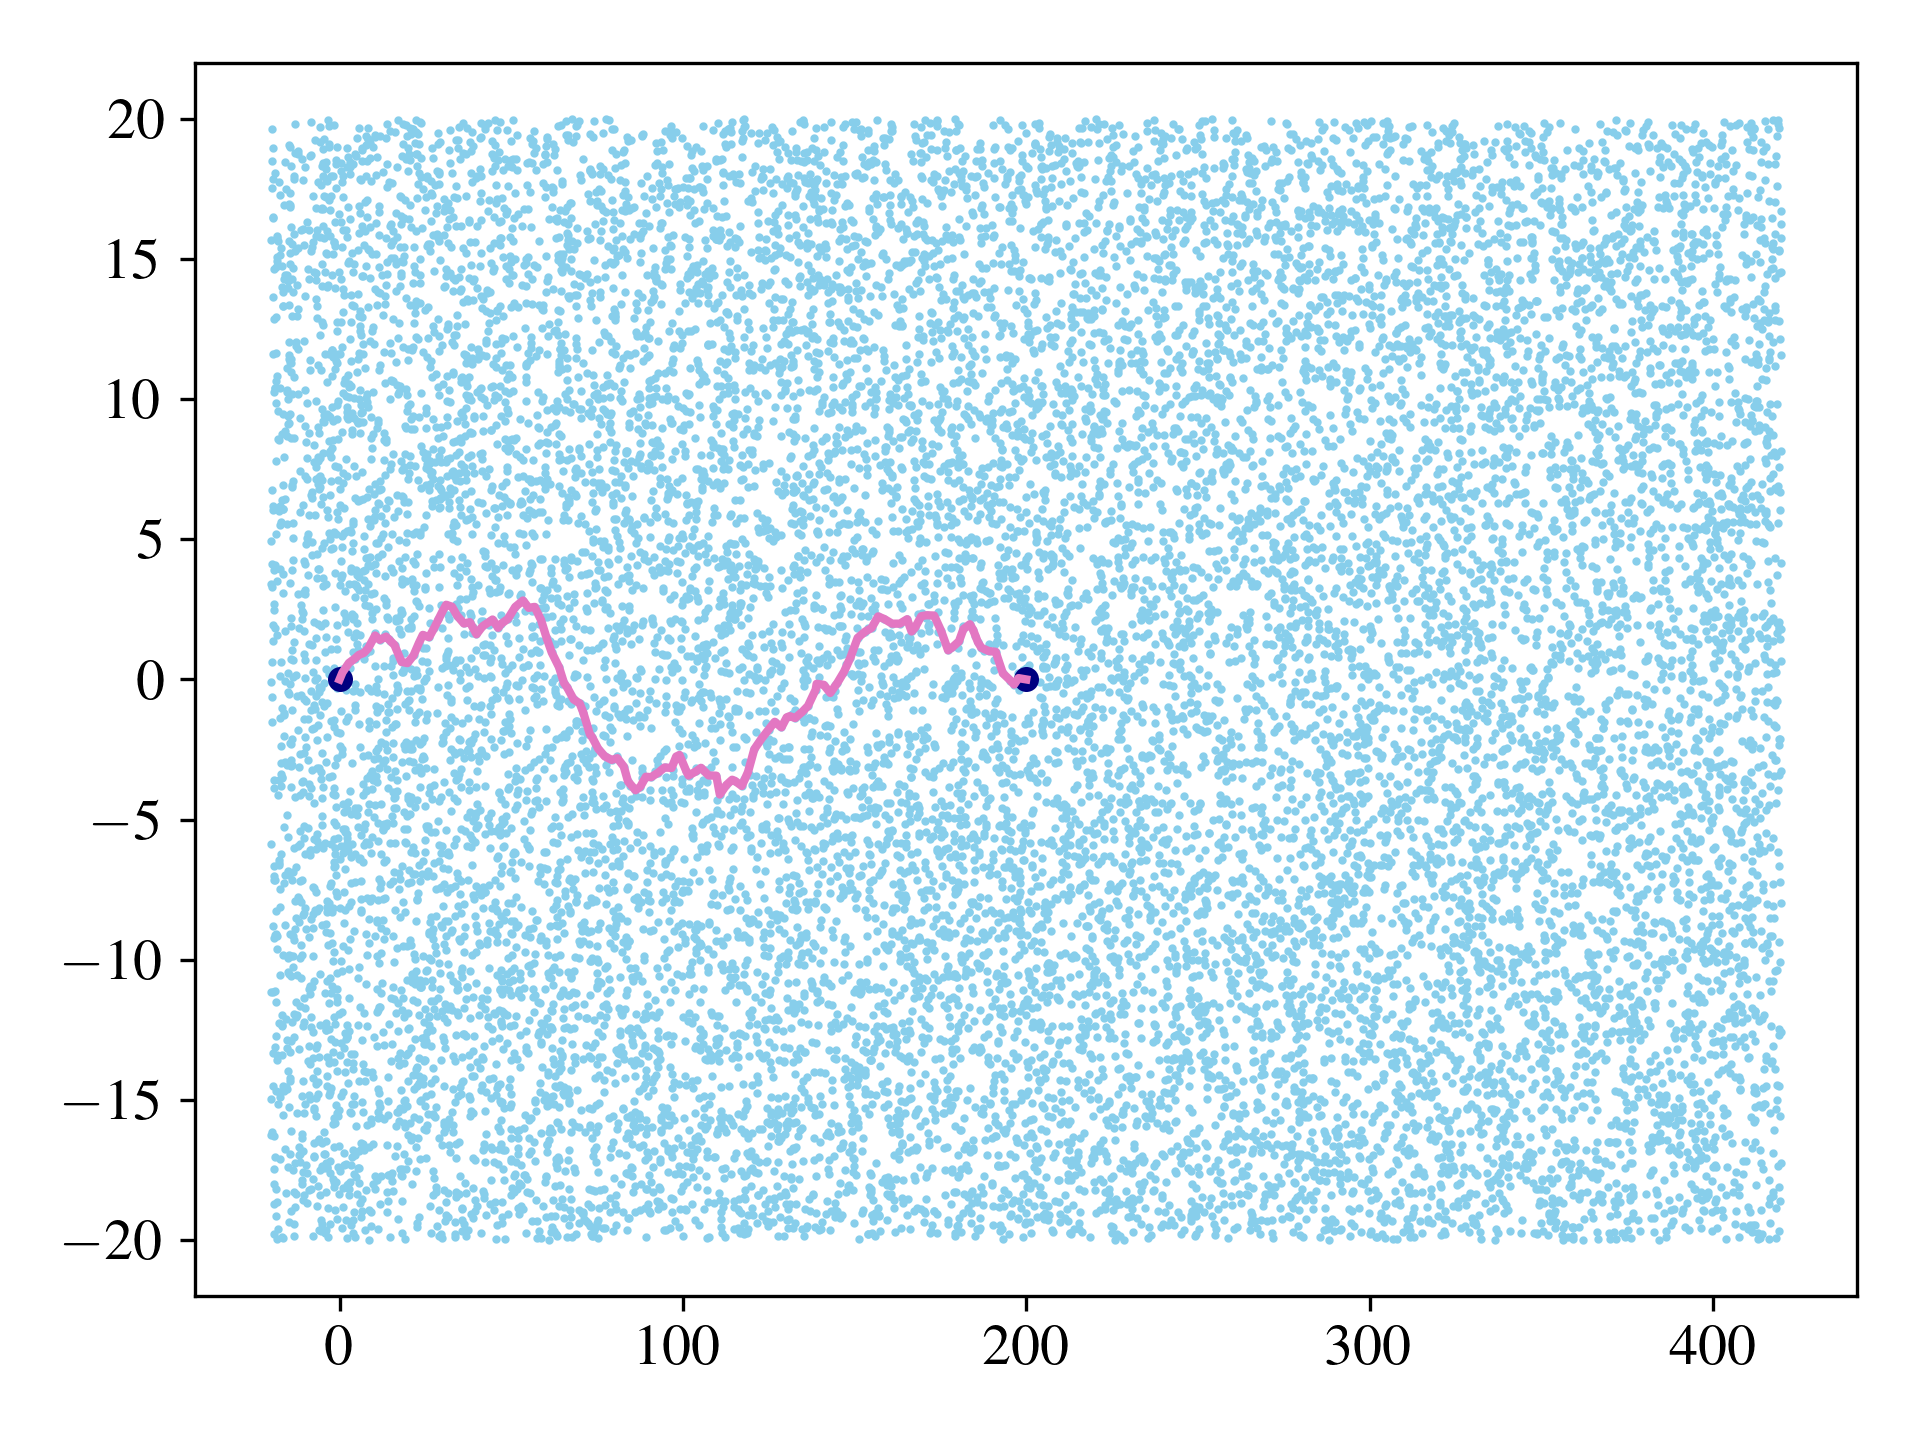
\includegraphics[width=0.3\textwidth]{atelier/path_2d_s-200}
\hfill
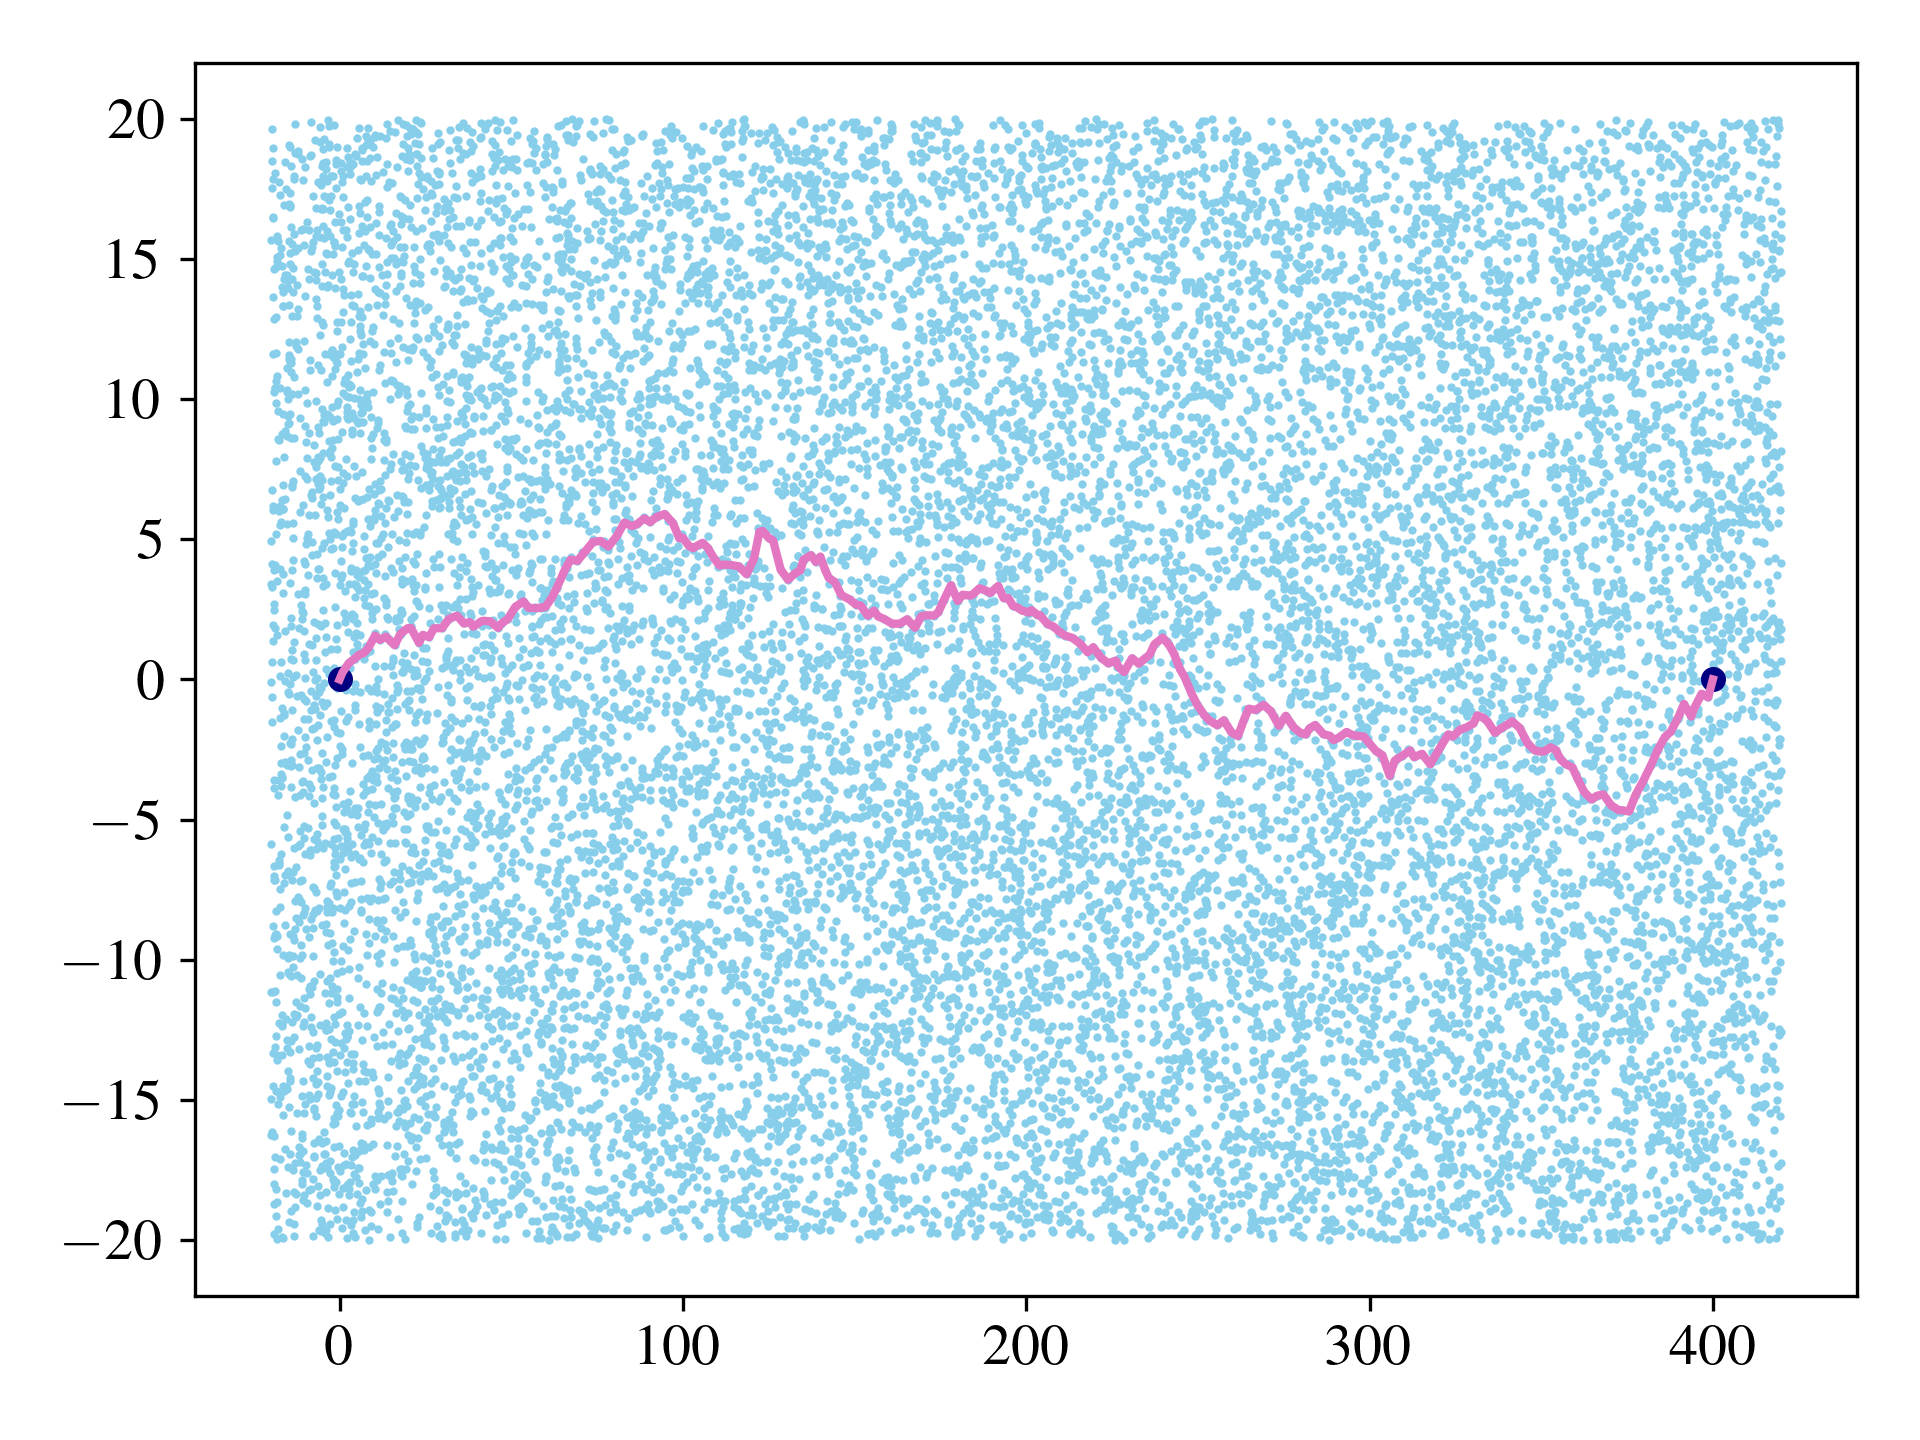
\includegraphics[width=0.3\textwidth]{atelier/path_2d_s-400}
\end{minipage}%

$s\mapsto h_s$ are growing step sizes with $h_s \gtrsim \log(s)^\frac{1}{d}$. 

% For slowly increasing $s\mapsto g(s)$ we have:
\alert{Approximate sub- and superadditivity}:
\begin{alignat*}{2}
    \Exp{T_{s+t}^\prime} &\leq \Exp{T_{s}^\prime} + \Exp{T_{t}^\prime} + g(s+t) \quad &&\text{\color{apple}\ding{52}\nc}
    \\
    \Exp{T_{2s}^\prime} &\geq 2 \Exp{T_s^\prime} - g(s) \quad &&\text{\color{grape}\textbf{???}\nc}
\end{alignat*}
% %
% \textbf{Subadditivity:} $\Exp{T_{s+t}^\prime} \leq \Exp{T_{s}^\prime} + \Exp{T_{t}^\prime} + g(s+t)$ \color{apple}\ding{52}\nc\\
% %
% \textbf{Superadditivity:} $\Exp{T_{2s}^\prime} \geq 2 \Exp{T_s^\prime} - g(s)$ \color{grape}\textbf{???}\nc
For \alert{ratio convergence} it suffices to freeze $h_s$:
\begin{align*}
\Exp{d_{h_s,\mathcal{X}_s}(0,2se_1)} \geq 2 \Exp{d_{h_s,\mathcal{X}_s}(0,s)} - g(s).
\end{align*}
%
With \alert{concentration of measure} we get \cite{bungert2022ratio}
%
\begin{block}{}
\begin{align*}
\abs{\frac{\Exp{d_{h_s,\mathcal{X}_s}(0,se_1)}}{\Exp{d_{h_s,\mathcal{X}_s}(0,2se_1)}} - \frac{1}{2}}
&\lesssim
\sqrt{\frac{\log(s)^{2/d}}{h_s}}\frac{\log(s)}{\sqrt{s}}\\
%
\Rightarrow \max_{\domain_n}\abs{\vec u_n - u} 
&\lesssim 
\log(n)^{2/9}\gres_n^{1/9}.
\end{align*}
\end{block}
\end{minipage}%
%
\hfill%
%
\begin{minipage}[b][\midHeight][t]{.31\textwidth}%
{\color{BaseDarkColor}\usebeamerfont{block title} Numerical Examples}\\
\begin{minipage}{.5\textwidth}%
\small%
Infinity harmonic function $u(x_1,x_2)=\abs{x_1}^{4/3}-\abs{x_2}^{4/3}$ on $\domain:=\{\abs{x_1}^{2/3}+\abs{x_2}^{2/3}\leq 1\}.$
\end{minipage}%
\begin{minipage}{.5\textwidth}%
\centering
{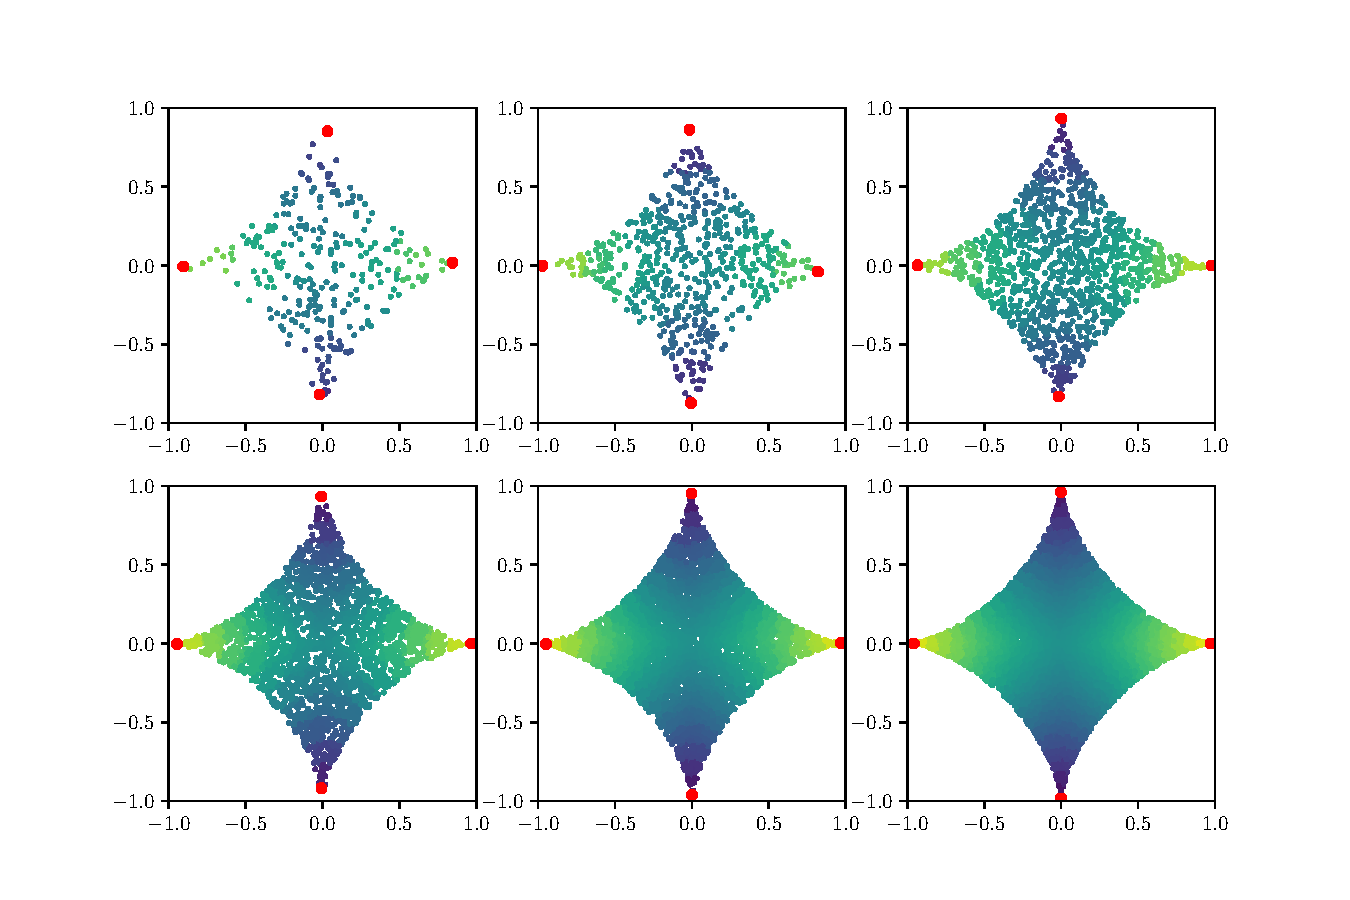
\includegraphics[width=0.8\textwidth,trim=1.8cm 1.1cm 1.8cm 1.4cm,clip]{atelier/neumann_star_solution}}%
\end{minipage}%
%
%
\vspace{.5em}

\begin{minipage}{.32\textwidth}%
\small
\centering%
AMLE rates for \hfill

$\eta(s)=\tfrac{1}{s}$:
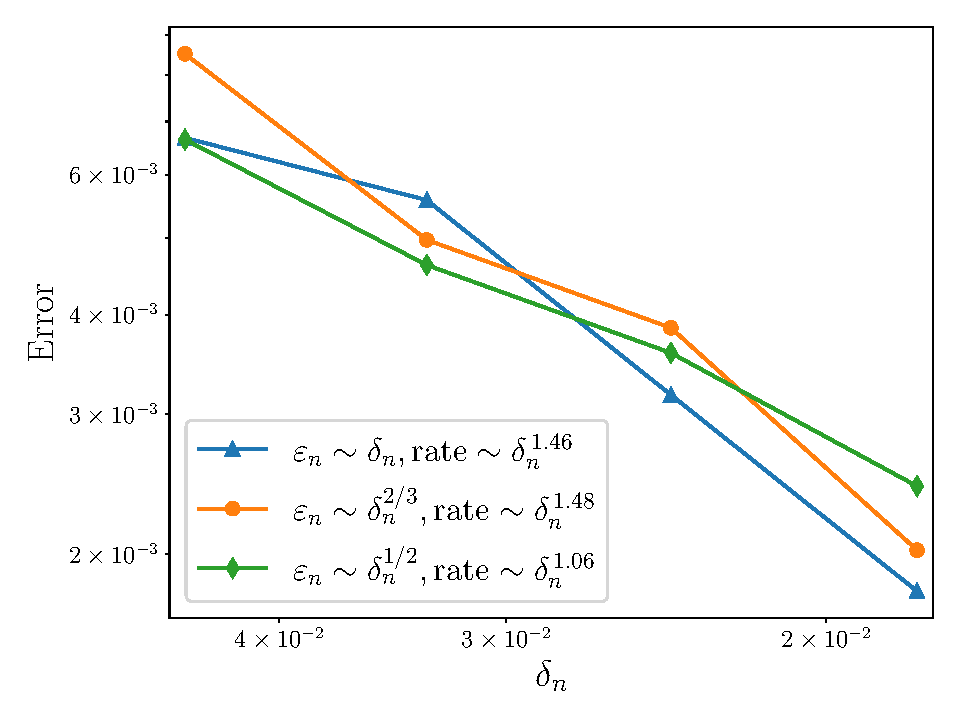
\includegraphics[width=1.02\textwidth]{atelier/aronsson_star_singular_plot}
\end{minipage}%
%
\hfill%
%
\begin{minipage}{.65\textwidth}%
\small
\centering
Ratio convergence rates for\\percolation length scales:
\vskip3pt%
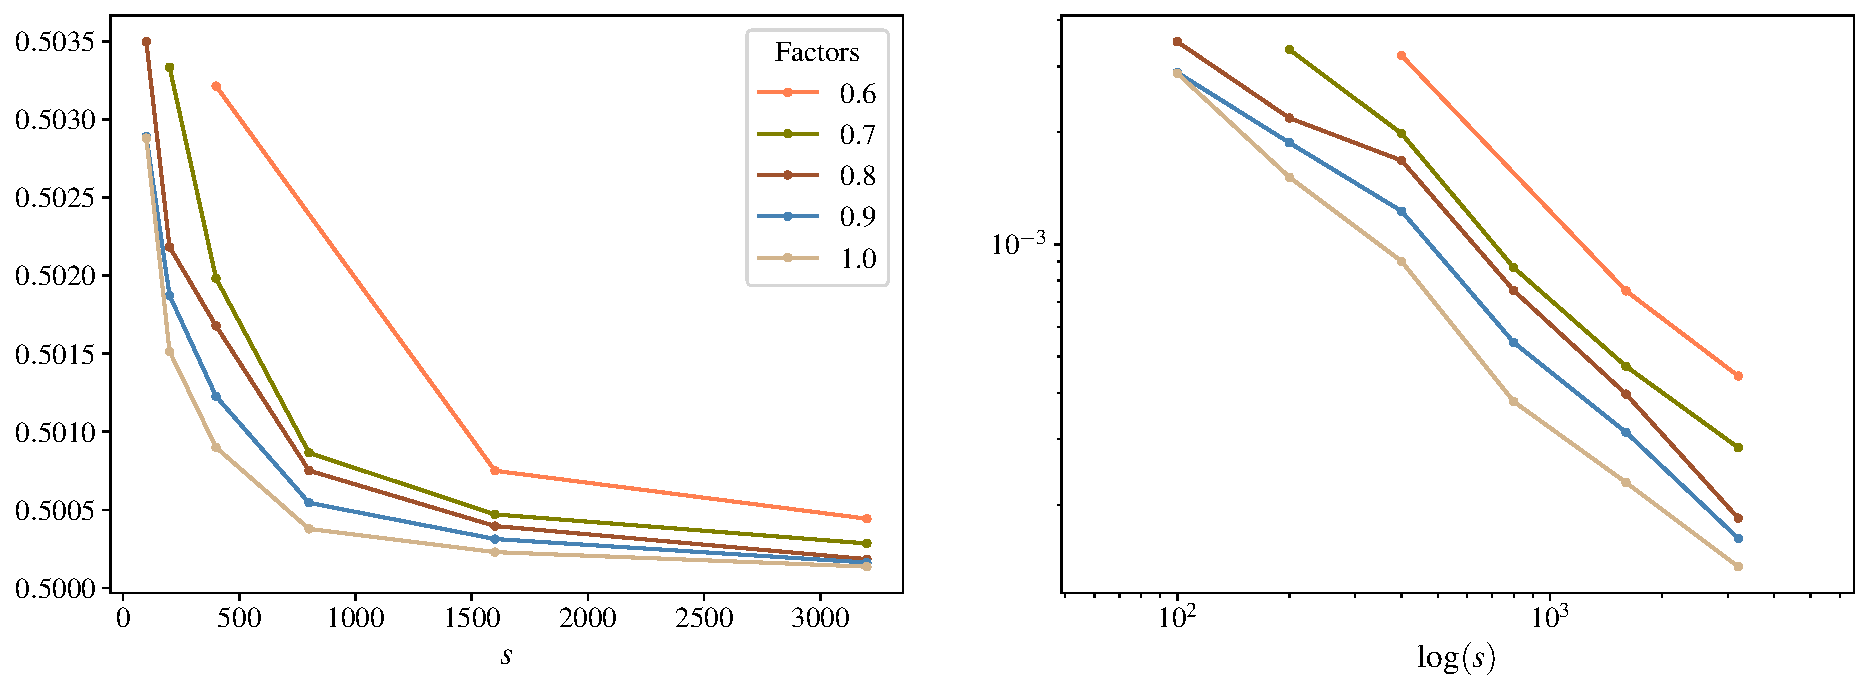
\includegraphics[width=\textwidth]{atelier/ratio_convergence_3d}%
\end{minipage}%
%
{\color{BaseDarkColor}\usebeamerfont{block title} References}
\AtNextBibliography{\tiny}%
\printbibliography[heading=none]


\end{minipage}%
%
\end{frame}
\end{document}